\documentclass[conference]{IEEEtran}

%%%%%%%%%%%%%%%%%%%%%%%%%%%%%%%%%%%%%%%%%%%%%%%%%%%%%%%%%%%%%%%%%%%%%%%%%%%%%%%%
%
% Package
%
%%%%%%%%%%%%%%%%%%%%%%%%%%%%%%%%%%%%%%%%%%%%%%%%%%%%%%%%%%%%%%%%%%%%%%%%%%%%%%%%
\usepackage{ifpdf}
\ifCLASSINFOpdf
  \usepackage[pdftex]{graphicx}
  % declare the path(s) where your graphic files are
  % \graphicspath{{../pdf/}{../jpeg/}}
  % and their extensions so you won't have to specify these with
  % every instance of \includegraphics
  \DeclareGraphicsExtensions{.pdf,.jpeg,.png}
\else
  % or other class option (dvipsone, dvipdf, if not using dvips). graphicx
  % will default to the driver specified in the system graphics.cfg if no
  % driver is specified.
  \usepackage[dvips]{graphicx}
  % declare the path(s) where your graphic files are
  % \graphicspath{{../eps/}}
  % and their extensions so you won't have to specify these with
  % every instance of \includegraphics
  \DeclareGraphicsExtensions{.eps}
\fi

\usepackage[utf8]{inputenc}
\usepackage[T1]{fontenc}
\usepackage[french, english]{babel}
\usepackage{cite}
\usepackage{caption}
\usepackage{amsmath,amsfonts,amssymb}
\usepackage{subcaption}
\usepackage{array}

\usepackage{float}
\usepackage{multicol}
\usepackage[]{algorithm2e}
\usepackage{hyperref}

%
% correct bad hyphenation here
\hyphenation{op-tical net-works semi-conduc-tor}

\DeclareMathOperator*{\argmin}{arg\,min}
\DeclareMathOperator*{\argmax}{arg\,max}

\begin{document}
%%%%%%%%%%%%%%%%%%%%%%%%%%%%%%%%%%%%%%%%%%%%%%%%%%%%%%%%%%%%%%%%%%%%%%%%%%%%%%%%
%
% Title
%
%%%%%%%%%%%%%%%%%%%%%%%%%%%%%%%%%%%%%%%%%%%%%%%%%%%%%%%%%%%%%%%%%%%%%%%%%%%%%%%%
\title{Correlation among smart grid actors}

%%%%%%%%%%%%%%%%%%%%%%%%%%%%%%%%%%%%%%%%%%%%%%%%%%%%%%%%%%%%%%%%%%%%%%%%%%%%%%%%
%
% Authors
%
%%%%%%%%%%%%%%%%%%%%%%%%%%%%%%%%%%%%%%%%%%%%%%%%%%%%%%%%%%%%%%%%%%%%%%%%%%%%%%%%
\author{Nicolas Gensollen, Monique Becker, Vincent Gauthier and Michel Marot  \\
\IEEEauthorblockA{CNRS UMR 5157 SAMOVAR, \\
Telecom SudParis/Institut Mines Telecom\\
Email: \{nicolas.gensollen, vincent.gauthier, michel.marot, monique.becker\}@telecom-sudparis.eu}}

\maketitle

%%%%%%%%%%%%%%%%%%%%%%%%%%%%%%%%%%%%%%%%%%%%%%%%%%%%%%%%%%%%%%%%%%%%%%%%%%%%%%%%
%
% Abstract
%
%%%%%%%%%%%%%%%%%%%%%%%%%%%%%%%%%%%%%%%%%%%%%%%%%%%%%%%%%%%%%%%%%%%%%%%%%%%%%%%%
\begin{abstract}
Achieving a successful energetic transition became a major goal for the 21st century in most developped countries. The reconciliation of several research areas and their recent focus on the same smart grid objective has led to major technical improvements. For instance, allowing large penetrations of renewables into the electricity production seemed more like a dream yesterday, but appears more and more doable as research progresses. The inherent volatility of some of these energy sources poses indeed various problems in such a constrained environment. It is often supposed that a large number of these small generators will be decentralized down to the distribution networks and even be owned by individuals. By enabling bi-directional flows, this vision revolutionises the nature of the simple today's consumer into some futuristic agent that can both consume and produce. Such an agent can obviously reduce its electricity bill by seeking energetic independance through demand side management programs coupled with storage. Nevertheless, as it could be the case that an agent's production exceeds its consumption and storage capacity, its ability to sell its extra-production appears as a way to save energy.

In this paper, we thus consider agents that tend to produce more than they consume and seek to sell their surplus of production. More precisely, we rely on aggregations of these agents that can be seen as virtual power plants with production and consumption components that are both variable. Because these virtual power plants are complex aggregations of different types of production means and consumption habits, the volatilities of the plants productions are deeply impacted by the correlation between the agents. We propose here an algorithm that takes the underlying correlation structure of the agents into account while forming the coalitions. We show then that the resulting diversified coalitions are able to generate higher benefits on a constrained energy market, and are more resilient to random failures of the agents.
\end{abstract}

\IEEEpeerreviewmaketitle


%%%%%%%%%%%%%%%%%%%%%%%%%%%%%%%%%%%%%%%%%%%%%%%%%%%%%%%%%%%%%%%%%%%%%%%%%%%%%%%%
%
% Section I: Introduction
%
%%%%%%%%%%%%%%%%%%%%%%%%%%%%%%%%%%%%%%%%%%%%%%%%%%%%%%%%%%%%%%%%%%%%%%%%%%%%%%%%
\section{Introduction}
\label{sec:introduction}

Designing stable power systems is a classical engineering challenge since blackout events can have catastrophic consequences. A recent approach introduced by complex systems theorists consists in abstracting the power grid as a graph where nodes represent loads, generators, or transformers, while edges stand for electrical lines. As graphs, power grids display some characteristics like clustering coefficients, degree distributions, or density for instance. These metrics enable scientists to get a better understanding of the structure of such complex systems. It appears that power grids are particular graphs compared to well-known large networks like the internet, the world wide web, or social networks. That is, they exhibit different characteritics, suggesting that they may behave differently. A common hypothesis for such a difference is that power grids are completely designed by a very small number of entities (electricity operators mainly), whereas other pre-cited graphs results from the interactions of billions of independant entities. Therefore, properties like power law degree distributions, prerential attachment, or hub oriented attacks do not necessarily apply with power grids.

Actually, drawing conclusions based only on the study of the underlying graph structure may lead to unrealistic results. Power grids are ideed dynamical systems governed by physical laws. Concepts such as shortest path or centrality metrics have thus to be extended to take into account the particular nature of power grids. Besides, stability and resilience of such systems are much more complex than the simple connectivity of the underlying graph. It is well-known for instance that frequency synchronization in the grid is a necessary condition for stability. A common solution consists in modeling the grid as a network of coupled oscillators governed by a swing equation dynamic. It can then be shown that the topology of the network impacts directly the capacity of the oscillators to reach the synchronized state.

Understanding power grids seems like a reasonable strarting point for studying so-called \textit{smart grids} that gained a lot of attention recently. As there exists many good articles presenting smart grid ideas, concepts, or architectures, we will not dwell too much on this point. In this paper, we rather concentrate on a different approach to the system stability. We consider a set of agents that are equiped with distributed energy ressources (DER) as well as electrical loads, such that an agent can produce and consume energy at any time. His production can be, of course, used to meet his own demand, but in cases where he is over-producing, we consider that he has the possibility to sell his extra-production to the grid. Such an agent model is known as a "\textit{prosumer}" (and will be called accordingly in this paper). 

The constraints necessary for the electrical grid to remain in a stable state obiously forbid any anarchic system where prosumers inject power whenever and however they want. An envisaged solution for organizing such a system consists in a market environement, where participating entities announce a production capacity for an upcoming period of time. These entities thus commit to injecting exactly at any time the contracted amount of power under financial penalities if they fail. Such a market system necessitates obviously some communication architecture to be viable. Since the number of prosumers in a system may be large, it seems unrealistic to have a flat centralized topology where a single agent coordinates all the others individually. Some articles suggest that a fully decentralized architecture will probably be too complicated to achieve, and that some kind of hierarchical hybrid topology seems more likely to be viable.

Moreover, taking into account that the production component of a prosumer is supposed to come mainly from renewables, its over-producing state, and therefore the power he injects in the grid, might be rather unstable.

It has been suggested that energy diversification, geographical expansion, as well as using storage devices are envisageable techniques for  stabilizing the production. Considering virtual coalitions of prosumers as potential providers, and allowing these aggregations to enter the market, could potentially solve some of these problems. Indeed, the system operator would only have to communicate with a relatively small number of aggregators, that in turn will use some internal communication protocol to manage the involved agents. Moreover, if the aggregation has been done properly, one should expect a more stable and predictable energy production for the coalition than for a single agent. This diversification idea is ideed a central topic of the present paper : given N prosumers, what coalitions should be formed so that the compromise between expected production and variability is optimized ?

We will see that variability in the coalitions productions can be quantified to a certain extend by the correlation among the agents forming the coalitions. Understanding the correlation reliationships among the agents can thus be illuminating in the sense that it will help us decide both what coalitions to form and how much they should sell. More precisely, we will build a framework in which the system operator has the possibility of fixing some entrance conditions on the market both in terms of stability and sufficient production. Based on predictions, coalitions can decide wether or not to enter and what power quantity they are willing to provide. Of course, coalitions failing at fulfilling their obligations during the contracted period of time (because of bad forecasts, unexpected rare events, or lying) will be exposed to financial penalities.

Because agents are susceptible to fail for diverse reasons, the impact on the system's stability is critical. The propensy of a system to undertake these failures is often refered to as its resilience. Once formed, we also investigate in this paper the resilience of the coalitions when prosumers fail. Despite the fact that loosing agents is always detrimental to the coalitions, we will see that, with our algorithm, coalitions tend to be less impacted by random failures.

The paper is organized as follows, section 2 will give a brief overview of the related litterature, section 3 will clarify how we generated realistic prosumer production traces based on weather data. In section 4, we will define most of the notations and explain why correlation between prosumer is a quantity of interest for our objective. Based on the conclusions of section 4, section 5 shows how we approached the problem in a complex system fashion. Finally, section 6 will provide some results both on performance of the method and resilience of the coalitions formed.


%%%%%%%%%%%%%%%%%%%%%%%%%%%%%%%%%%%%%%%%%%%%%%%%%%%%%%%%%%%%%%%%%%%%%%%%%%%%%%%%
%
% Section II: Related Work
%
%%%%%%%%%%%%%%%%%%%%%%%%%%%%%%%%%%%%%%%%%%%%%%%%%%%%%%%%%%%%%%%%%%%%%%%%%%%%%%%%

\section{Related Work}
\label{sec:related}

The intermittent nature of renewables such as wind or solar power introduces new challenges in control design. Besides, on the contrary to fossil plants whose production can be scheduled in advance to meet the expected consumption, renewables by definition only produce when the natural ressource is present. Unfortunately, these moments do not necessarily coincide with the consumption peak hours. A first approach to remedy this situation by acting on the consumption component is the use of dynamic ectricity prices sent to the end users. Together with demand side management techniques implemented on the smart meters, they consitute a first tool for shaping the consumption profiles. In periods where the production is expected to be greater than the consumption, prices are scheduled low in order to encourage end users to delay their elastic loads to these periods. On the contrary, when the production is expected to be less than the consumption, high prices are scheduled to deter any delayable loads over these periods.

Another popular approach on the production side, is to combined renewable generators with storage devices, such that these are charged when there is a surplus of production, and discharged when the consumption exceeds the production. Although simple, this idea causes numerous challenges. Depending on the size of the system considered, centralized or decentralized control is desirable. In[], the authors introduce a distributed energy management system with a high penetration of renewables such that power is scheduled in a distributed fashion. In [] the optimal storage capacity problem is adressed. There is indeed an interesting tradeoff between the costs of the equipments and the expected availability of power. The authors develop a framework that enables them to exhibit a Pareto front of efficient solutions.

Although there are great progresses in stabilizing the production by demand side managment or storage architectures, the need for good prediction techniques is more important than ever. Understanding the statistical properties of wind or solar irradiance are already well-established areas of research. There exists indeed a very interesting litterature on techniques aiming at predicting wind or solar irradiance profiles for future periods with error margins. In this paper, we adopt a slightly different approach : we suppose that the agents have historical records of their production and consumption, and we seek aggregations of agents with high expected production and low variability (wich is sometimes called risk in the present paper).

Optimization of expected returns to risk is a traditional goal in finance. It is indeed well-known, that the more risk one is willing to take, the higher his potential gains. On the contrary, when investing exclusively on low rik assets, one should expect relatively small gains. This tradeoff is formalized in the Markowitz' portfolio theory. More precisely, given a set of assets for which we have some historic data of returns, the objective is to find a linear combination of these assets (the so-called portfolio) which maximizes the expected value while minimizing the variance of the portfolio's return. Markowitz's answer is a set of efficient portolios that all optimize in some sense this tradeoff. If one is able to put a number on his risk acceptance or on the target expected return, the corresponding efficient portfolio is a priori the best option. 

This problem exhibits similarities with our objective of forming stable coalitions since our expected return can be formulated as the expected production and the risk / volatility as the variance of the production. However, one of the assumptions in the portfolio theory is that returns are normaly distributed random variables (or at least that the joint distribution is elliptic). In this paper, we chose to use normal distributions only for explanation purposes, or for estimating some parameters. Therefore, all the results are computed based on observed distributions (sometines far from gaussians).

One of the key point in the Markowitz theory is to consider explicitely the correlation structure between the assets since these correlation relationships impact directly (as we will see in section X) the variances of the portfolios. Since the work of Mantanega, an interresting approach consists in computing a distance metric based on the correlation coefficients in order to organize the series in a correlation graph where the weight of an edge between two timeseries (nodes) is the metric value for these series.

Because the metric can be computed for all pairs, these graphs are complete and of little use as is. Historically, the approach used by Mantanega was to compute a minimum spanning tree over the correlation graph as to extract a correlation structure of the form of a hierarchical clustering. Later on, it was pointed out that, by definition, a spanning tree could not capture the underlying clustering structure hidden in the correlation graph. Another filtering approach by mean of a threshold $ \epsilon $ on the edge weights solves this problem and allows one to exhibit clusters of correlated series. In the following we will refer to these filtered graphs as $ \epsilon $-graph.

An efficient portfolio of assets and a clustering of assets based on the correlations are obviously two very distinct things. And none of them is exactly what we seek. We will see in section X, how we combined both theories in order to form sufficiently producing coalitions with an acceptable volatility level.

%%%%%%%%%%%%%%%%%%%%%%%%%%%%%%%%%%%%%%%%%%%%%%%%%%%%%%%%%%%%%%%%%%%%%%%%%%%%%%%%
%
% Section III: Generating realistic prosumer patterns
%
%%%%%%%%%%%%%%%%%%%%%%%%%%%%%%%%%%%%%%%%%%%%%%%%%%%%%%%%%%%%%%%%%%%%%%%%%%%%%%%%

\section{Generating realistic prosumer patterns}
\label{sec:data}

An essential component of the smart grid is the smart meter which makes the interface between the end user and the rest of the system. Smart meters coupled with sensors measure quantities of interest (like instantaneous consumption), receive informations from the grid (electricity price for instance), and take actions accordingly (demand side management program). Smart meters are currently and gradually deployed, and will probably provide interesting datasets to work on. Unfortunately, at the time this paper was written, production and consumption data for prosumers over a large region were not yet available to our knowledge. Some interesting experiments are notwithstanding being conducted and data are progressively made public []. 

In the following, we denote by $ P_{i}(t) $ the instantaneous extra-production of agent i at time t :

\begin{equation}
P_{i}(t) = P_{i}^{P}(t) - P_{i}^{D}(t)
\end{equation}

Where $ P_{i}^{P}(t) $ represents the total production of agent i at time t and $ P_{i}^{D}(t) $ its consumption at time t. In other words, $ P_{i}(t) $ represents the instantaneous surplus of power that agent i is willing to sell at time t. As explained above, since large datasets containing this quantity over time are not yet available, we simulated these traces by considering separately $ P_{i}^{P} $ and $ P_{i}^{D} $.

For a prosumer i, it is possible to write both quantities as a sum over the distributed energy ressources ($ DER_{i} $) and loads ($ load_{i} $) of i : 

\begin{equation}
P_{i}^{P}(t) = \sum_{k \in DER_{i}} P_{k}(t)
\end{equation}
\begin{equation}
P_{i}^{D}(t) = \sum_{k \in load_{i}} P_{k}(t)
\end{equation}

For simplicity, in this paper we only consider windturbines (WT) and photovoltaic panels (PV) as possible DER for the agents ($ DER_{i} = WT_{i} \cup PV_{i} $):  

\begin{equation}
P_{i}^{D}(t) = \sum_{k \in WT_{i}} P_{k}(t) + \sum_{k \in PV_{i}} P_{k}(t)
\end{equation} 

We denote by $ \nu_{i}(t) $ and $ \xi_{i}(t) $ the wind speed (in $ m.s^{-1} $) and the solar irradiance ( in $ W.m^{-2} $) at the location of agent i and at time t, so that :
\begin{equation}
 P_{i}^{P}(t) = \sum_{k \in WT_{i}} \mathcal{F}_{WT}( \nu_{i}(t) ) + \sum_{k \in PV_{i} } \mathcal{F}_{PV}(\xi_{i}(t) ) 
\end{equation}
Where $ \mathcal{F}_{WT} $ (resp. $ \mathcal{F}_{PV} $) is the power curve for the windturbines (resp. photovoltaic panels). We made here the implicit assumption that all windturbines (resp. photovoltaic panels) have the same power curve. The model can be easily extended to muplitiple power curves accounting for different types of generators. More details about power curves and their approximations can be found in []. 

Weather quantities like wind speed or solar irradiance appear thus as alternative data for generating the $ P_{i} $ series. Fortunately, these kind of data are easier to find, and since the developement of small personal weather stations, their geographical granularity keeps increasing.  A quantity like wind speed depends both on time and location (we neglect height since this information is rarely present in the data). In the following, time is discretized into slots and space into zones. A zone is simply a portion of the considered space for which we have weather data. Therefore, if prosumers i and j are positioned on the same zone, they are exposed to the same weather. Adding some intra-zone noise can easily be done though not considered in this paper. The process for generating the $ P_{i} $ series is pictured in the first block of the process diagram (see figure \ref{fig:process}).

\begin{figure}
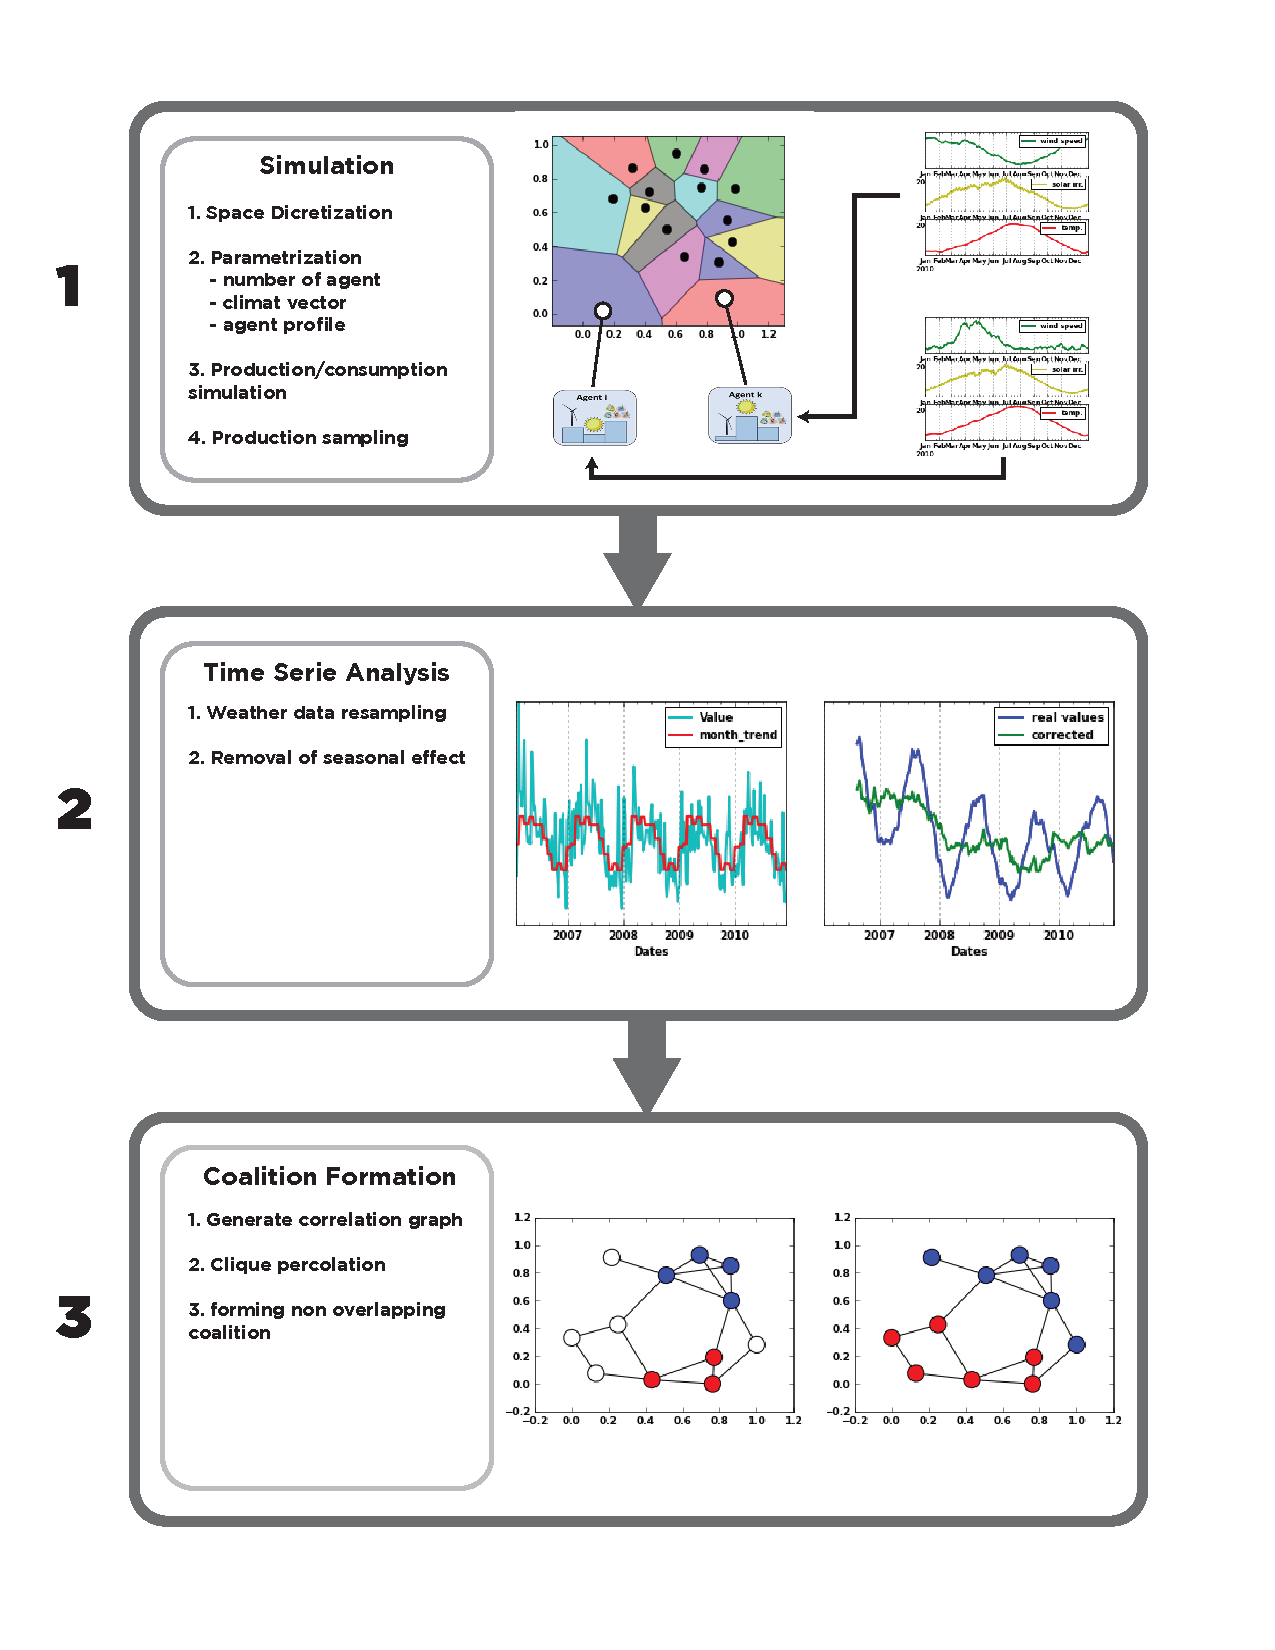
\includegraphics[scale=.45]{Fig2.pdf}
\caption{Process diagram}
\label{fig:process}
\end{figure}

Note that a prosumer i is defined by his zone $ Z_{i} $ as well as the sets $ DER_{i} $ and $ load_{i} $. That is, a prosumer can be configured to represent anything from a single windturbine for instance ($ DER_{i} = \{ WT_{0} \} $ and $ load_{i} = \emptyset $) to a pure load ($ DER_{i} = \emptyset $ and $ load_{i} = \{ L_{0} \} $) through more complex combinations. In practice, we use random configurations for the agents.

In the rest of the paper, we use french weather data (see www.infoclimat.fr) starting in january 2006 and ending in december 2012, with a sampling frequency of three hours, and generate N timeseries of extra-production over this date range.



%%%%%%%%%%%%%%%%%%%%%%%%%%%%%%%%%%%%%%%%%%%%%%%%%%%%%%%%%%%%%%%%%%%%%%%%%%%%%%%%
%
% Section III: Model
%
%%%%%%%%%%%%%%%%%%%%%%%%%%%%%%%%%%%%%%%%%%%%%%%%%%%%%%%%%%%%%%%%%%%%%%%%%%%%%%%%

\section{Notations}
\label{sec:notations}

This section provides most of the notations and introduces important concepts for the rest of the paper. As explained in section \ref{sec:data}, we consider a set $ \mathcal{A} = \{a_{1},a_{2},...,a_{N} \} $ of N prosumers configured randomly, and for each agent, we simulate its extra-production $ P_{i}(t),\ \forall i \in \mathcal{A} $ from 2006 to 2012. Based on these historical values, our objective is now to form groups of prosumers (the so-called coalitions) so that the global power production resulting from the superposition of individual's extra-productions be both sufficiently high and predictable. Let $ P_{S}(t) = \sum_{i \in S} P_{i}(t) $ be the extra-production of coalition S at time t. 

Suppose now that coalition S has to suggest a production value $ P_{S}^{CRCT} $ to enter the market. This means that, during the time S is on the market, it will have to inject in the grid exactly $ P_{S}^{CRCT} $ at any time t and will be rewarded proportionally to this amount, with penalities if it deviates. Obviously, the actual extra-production will not be constant at this value and will oscillate due to intermittencies in the production and consumption. If S always produces more than $ P_{S}^{CRCT} $, it will never have to pay penalities, but it is losing some gains since it could have annonced a higher contract value. If the production oscillates around $ P_{S}^{CRCT} $, by using batteries or demand side management techniques (see section \ref{sec:related}), S could be able to maintain its production to the contract value at any time. Nevertheless, if the oscillations are too important compared to the available storage capacity, S will probably break the contract and pay penalities. We can see that there is a return over risk tradeoff here, meaning that coalitions should find the right balance between announcing too low and losing some potential gains, and claiming too high and paying penalities. 

Let us illustrate the rest of the notations and concepts with a simple example. We consider only two agents i and j such that the distribution of their extra-production can be approximated by normal distributions : $ P_{i} \sim \mathcal{N}(\mu_{i}, \sigma_{i} ) $ and $ P_{j} \sim \mathcal{N}(\mu_{j}, \sigma_{j} ) $. This is only for explanation purposes as it is of course rather unrealistic in real situations where the distributions are skewed. Using simple statistics, we can write the distribution of the coalition $ S = \{i,j\} $ as $ P_{\{i,j\}} \sim \mathcal{N}(\mu_{ij}, \sigma_{ij}) $, where :

\begin{equation}
\left\{ \begin{array}{lll}
		\mu_{ij} = \mu_{i} + \mu_{j} \\
		\sigma_{ij} = \sqrt{\sigma_{i}^{2} + \sigma_{j}^{2} + \rho_{ij} \sigma_{i} \sigma_{j} }
\end{array} \right.
\end{equation}

$ \rho_{ij} $ being the Pearson's correlation coefficient between $ P_{i} $ and $ P_{j} $. If the coalition $ \{i,j\}$ proposes a contract value $ P_{S}^{CRCT} $, all instants where $ \{i,j\}$ will produce less than $ P_{S}^{CRCT} $ is critical. Indeed, in this kind of situations, $ \{i,j\}$ will either have to discharge batteries to keep up with its contract, or pay penalities to the grid. The probability that $ \{i,j\}$ is underproducing compared to the contract : $ Pr[P_{i,j} \leq P^{CRCT}] $ is thus an important indicator of the coalition's quality. A well-known result for normal distributions is that the cumulative distribution function can be written as :
\begin{equation}
Pr[P_{ij} \leq P_{S}^{CRCT}] = \dfrac{1}{2} \left[ 1+ erf \left( \dfrac{P_{S}^{CRCT} - \mu_{ij}}{\sigma_{ij}\sqrt{2}} \right) \right] 
\end{equation}
 
Where $ erf $ is the error function : $ erf(x) = \dfrac{2}{\sqrt{\pi}}\int_{0}^{x} e^{-t^{2}} dt $.

The amount of risks a given coalition is willing to take depends on a lot of things, among wich its capacity to compensate for under-producing (using batteries, backup generators...), or the risk aversion of the aggregator. Selecting the right contract value appears thus as an interesting problem on its own that we plan to investigate in future works. In order to keep the present paper in a reasonable length, we simplify the contract value selection problem a little bit by giving some responsabilities to a third party named the grid operator. The role of the grid operator is to constrain the market entry to coalitions able to propose both sufficiently high and sufficiently credible contract values. More formally, let $ \phi \in [0,1] $ be the reliability threshold fixed by the grid operator as a maximum value for the probability of under-producing. The highest contract value that a coalition can propose is thus $ P_{S}^{CRCT \star} $ such that $ Pr[P_{ij} \leq P_{S}^{CRCT \star}] = \phi $. In the gaussian example, this translates by coalition $ \{i,j\}$ announcing :

\begin{equation}
\label{eq:P_star}
P_{S}^{CRCT \star} = \mu_{ij} - \sqrt{2} \sigma_{ij} erf^{-1}( 1 - 2 \phi )
\end{equation}

\begin{figure}
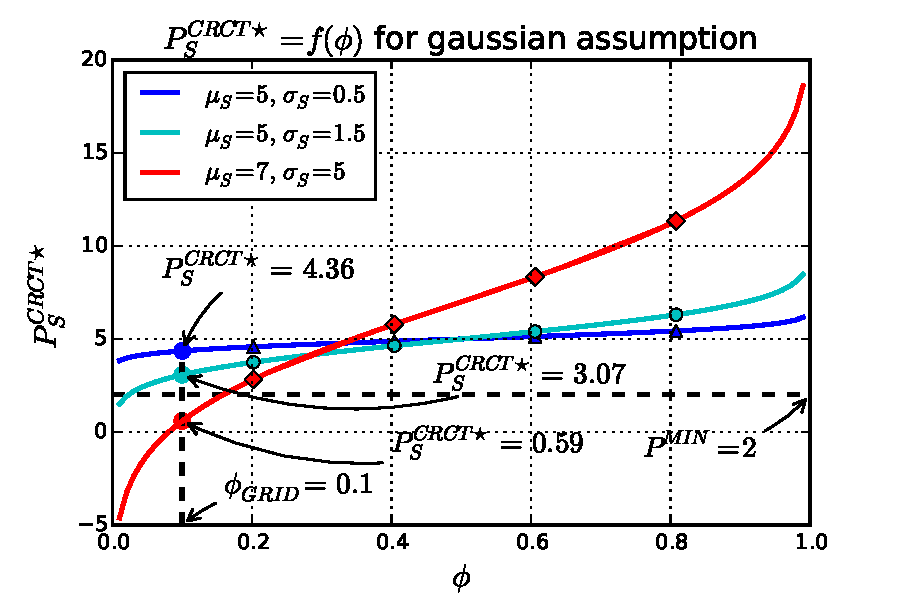
\includegraphics[scale=.6]{gaussian_P_star.pdf}
\caption{$ P_{S}^{CRCT \star} $ depending on reliability parameter $ \phi $ for gaussian distributions (see equation \ref{eq:P_star}). Blue curve with triangles stands for a coalition S with an expected production of 5 units and a standard deviation of 0.5. Under a grid policy of $ \phi = 0.1 $, it is able to announce a contract value of $ P_{S}^{CRCT \star} = 4.36 $. The same coalition in term of expected production ($\mu = 5 $), but with a higher variance ($ \sigma = 1.5 $, cyan curve with circles) can only afford a smaller contract value of $ P_{S}^{CRCT \star} = 3.07 $. The red curve with diamonds stands for a coalition with a higher expected production $(\mu = 7)$, but with a very high unpredictability ($ \sigma = 5 $). For low values of $ \phi $, this coalition is thus heavily penalized and can only afford a contract of $ 0.59 $ units. Under grid policy $ (\phi = 0.1, P^{MIN} = 2) $, this last coalition is thus not allowed to enter the market (red dot below the horrizontal dashed line). }
\label{fig:Gaussian}
\end{figure}

This is the best contract value that the coalition S can afford giving the stability policy $\phi$ of the grid operator. Figure \ref{fig:Gaussian} shows how $ P_{S}^{CRCT \star} $ evolves according to the reliability parameter $ \phi $. For illustration, the range of $ \phi $ values is shown from 0 to 1, but in practice, only small values of $ \phi $ really make sense : $ \phi = 1 $ for instance means that coalitions can announce absolutely anything since the probability of producing less than any contract value is necessarily less than one by trivial definition of a probability. As visible on figure \ref{fig:Gaussian}, coalitions with high expected productions but presenting a high unpredictability are penalized and can only afford small contracts.  

In order not to overload the market with unrealistically small coalitions, the grid operator also specify a lower bound $ P^{MIN} $ on the contract values. We thus characterized a valid coalition as one satisfying the two conditions :

\begin{equation}
\left\{ \begin{array}{lll}
			Pr[P_{ij} \leq P_{S}^{CRCT}] \leq \phi \\
			P_{S}^{CRCT} \geq P^{MIN}
\end{array} \right.
\end{equation}

On figure \ref{fig:Gaussian}, $ P^{MIN} $ is fixed to 2 units for illustration purpose. For $ \phi = 0.1 $, only blue triangles and cyan circles coalitions are valid while red diamonds coalition is not.

The gaussian assumption of this small example is convenient as it allows us to write $ P_{S}^{CRCT \star} $ analytically. Nevertheless, such assumption is rather unrealistic in practice. In the following, we keep the same framework but release this gaussian assumption unless the contrary is specified. This assumption will indeed be convenient for computing some parameter estimates.

%%%%%%%%%%%%%%%%%%%%%%%%%%%%%%%%%%%%%%%%%%%%%%%%%%%%%%%%%%%%%%%%%%%%%%%%%%%%%%%%
%
% Section V: Coalition Formation
%
%%%%%%%%%%%%%%%%%%%%%%%%%%%%%%%%%%%%%%%%%%%%%%%%%%%%%%%%%%%%%%%%%%%%%%%%%%%%%%%%

\section{Coalition Formation}
\label{sec:forming}

Now that we defined the notions of contract values and valid coalitions, we can face the problem of forming the "right" coalitions given a pool of agents. In this paper, we consider the "right" coalitions as being the ones that maximize some utility notion that, basically, indicates how much stable power can be injected in the grid. This section aims at formalizing this utility notion, while explaining how this utility will be optimized in a greedy fashion over the correlation structure of the agents. 


\subsection{Utility function}

We designed our model in a way that coalitions are remunerated proportionnally to their contract values $ \mathcal{U}(S) \propto P_{S}^{CRCT} $. That is, if $ \lambda $ is the unitary price rate for electricity, a coalition S injecting $ P_{S}^{CRCT} $ in the grid during a period $ [t_{0},t_{k}] $ earns :

\begin{equation}
\mathcal{U}(S ) = \int_{t_{0}}^{t_{k}} \lambda P_{S}^{CRCT} dt = P_{S}^{CRCT} \lambda \Delta_{t}
\end{equation} 

Since $ \lambda $ appears, in this simple model, just a multiplicative constant, we consider for simplicity $ \lambda = 1 $ in the following. The utility of S is now the amount of energy S plans to inject during its contract period. Since we focused on power quantities from the begining of the present paper, and because the power injected by S in the grid is supposed to be constant over time, we simplify further the utility to its contract value : $ \mathcal{U}(S) = P_{S}^{CRCT} $. Although concise, this formulation suffers a major drawback. It is indeed not a concave function, meaning that coalitions can grow as large as the number of agents allows it, without any counterparty. 

Such a model, that virtually allows infinitely large coalitions, is in practice not realistic. There are indeed costs (communication costs for instance) that increase with the coalitions sizes. We take this observation into account by rescaling the utility of a coalition S by its size in term of number of agents ($|S|$):

\begin{equation}
\mathcal{U}(S) = \left\{ \begin{array}{lll}
							\dfrac{1}{|S|^{\alpha}} \dfrac{ P_{S}^{CRCT} }{P^{MAX}},\ if\ S\ is\ valid, \\
							0,\ if\ S\ is\ not\ valid
						 \end{array}
				  \right.
\end{equation}

Where parameter $ \alpha $ controls to what extent the size of the coalition impacts its utility, and $ P^{MAX} $ is a normalizing factor. $ P^{MAX} $ can be seen as the maximum production which can be injected in the grid.

Based on $ \mathcal{U} $, the marginal contribution of an agent i can be expressed as $ \delta_{S}(i) = \mathcal{U}(S+\{i\}) - \mathcal{U}(S) $. A coalition S has thus an interest in adding an additional agent i if this marginal contribution is positive : 

\begin{equation}
\delta_{S}(i) \geq 0 \Leftrightarrow P_{S+\{i\}}^{CRCT} \geq P_{S}^{CRCT} \left( \dfrac{|S|+1}{|S|} \right)^{\alpha}
\label{eq:marginal_benefit}
\end{equation}

If $ \alpha $ is set to zero, agents are added as long as they increase the contract value of the coalition. If $ \alpha $ is greater than zero, additional agents have to increase the contract value by some factor. Since tunning the utility function with $ \alpha $ is not necessarily convenient, we relate $ \alpha $ to the mean sizes of the coalitions $ \bar{N} $. If we wish that $ \mathcal{U}(S) $ tends to form coalitions of size approximately of the order of $ \bar{N} $, then :

\begin{equation}
\left[ \dfrac{\partial{ U}}{ \partial{|S|}} \right]_{|S| = \bar{N}} = 0
\label{eq:derivative}
\end{equation}

In order to get an estimator for $ \alpha $, we solve equation \ref{eq:derivative} in a gaussian case (as in section \ref{sec:notations}). Furthermore, since considering all the possible interactions between agents is analytically intractable, we use here a mean approximation. Any quantity x that varies over the agent set is thus simplified in its mean value $ \bar{x} $. Solving equation \ref{eq:derivative} for $ \alpha $ in these conditions yields :

\footnotesize
\begin{equation}
\alpha^{\star}_{\bar{N}} = \dfrac{0.7 \bar{\sigma}(\bar{\rho}-1)erf^{-1}(2 \phi - 1)}{\bar{\mu}\sqrt{\bar{N}(\bar{\rho}\bar{N}-\bar{\rho}+1)}+1.4 \bar{\sigma} erf^{-1} (2 \phi -1 ) (\bar{\rho}\bar{N}-\bar{\rho} + 1)} 
\label{eq:alpha_star}
\end{equation}
\normalsize

Figure \ref{fig:mean_approx} shows how $ \alpha^{\star} $ and the utility function evolves according to the mean size of the coalitions $ \bar{N} $. These nice curves are of course only valid in the simplified example considered here, but they will provide some guidance when using real data.

\begin{figure}
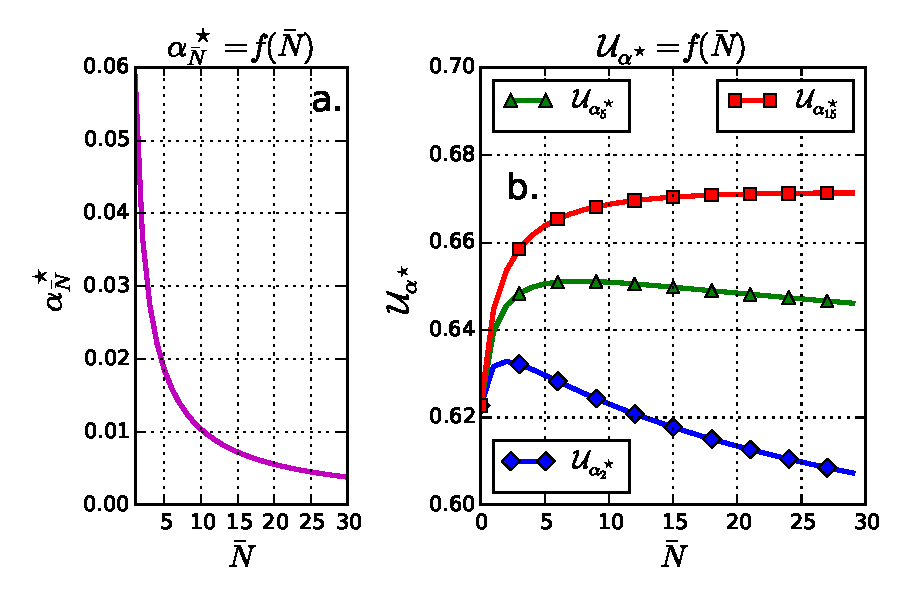
\includegraphics[scale=.6]{mean_field.pdf}
\caption{Gaussian mean approximation. Subplot \textbf{a} shows how the parameter $ \alpha $ of the utility function should be chosen in function of the mean desired size of the coalitions (see equation \ref{eq:alpha_star}). Subplot \textbf{b} dislays the corresponding utility functions for different values of $ \alpha $. Blue curve with diamonds favors very small coalitions of 2 agents while the green one with triangles favors 5 agents coalitions. Finally, the red curve with squares has an optimum size of 15 agents. }
\label{fig:mean_approx}
\end{figure}

%Clearly, if $ \alpha = 0 $, whatever the size of the coalition, additional agents are added as long as they increase the contract value. Values of $\alpha $ greater than zero implies that additional agents must improve the contract value by a certain coefficient that decreases and converges to one as the size of the coalition is growing. For instance, if $\alpha = 1$ and $ |S| = 1 $, an additional agent must first double the contract value to be included, the next agent will then have to increase it by a factor of $ 1.5 $, and so on... Obviously, $ \alpha $ impacts directly the sizes of the coalitions formed. In the following, we consider the case where $ \alpha = 1 $.

As can be pointed out, the purpose of $ \mathcal{U} $ is not a study of coalitions stability against player defection, wich game theory provides a lot of tools for. This is indeed a problem on its own. The redistribution of a coalition's utility in terms of individual payoffs will therefore not be considered directly in this paper. $ \mathcal{U} $ can be rather interpreted as a measure of how good a given coalition is according to our criteria since it favors coalitions with good production to risk ratios.


\subsection{Representing the correlation structure}

\subsubsection{Filtering the correlation graph}

The previous section explained that coalitions with small variances in their production probability distributions are more likely to afford better contracts. Furthermore, the gaussian approximation highlighted that the correlation structure of the agents plays an important role in finding stable coalitions. Usually, this correlation structure is formalized with a covariance matrix or a correlation matrix that contains all the correlation coefficients between the agents : $ M = (\rho_{ij})_{\forall i,j \in \mathcal{A}^{2}}$.

In the following, we use two opposite distance metrics : 

\begin{equation}
\left\{ \begin{array}{lll}
			d_{ij}^{1} = 1 - \rho_{ij}^{2}, \\
			d_{ij}^{2} = \rho_{ij}^{2} = 1 - d_{ij}^{1}
\end{array} \right.
\end{equation}

Clearly, $ d^{1} $ (resp. $ d^{2} $) maps two correlated series as close points (resp. distant) while two uncorrelated series are distant (resp. close). These metrics enable us to compute a correlation graph $ G_{1} = (\mathcal{A}, E_{1}) $ and a "de-correlation" graph $ G_{2} = (\mathcal{A}, E_{2} ) $. For any i and j, the weight of the edge $ e_{ij} $ is $ d_{ij}^{1} $ in $ G_{1} $ and $ d_{ij}^{2} $ in $ G_{2} $.

Selecting the right filter $ \epsilon $ for the $ \epsilon $-graph is an important point since it affects the correlation structure which affects in turn the formation of the coalitions. Unfortunately, there seems to be no clear consensus in the litterature on how to select such a threshold. We will see later in this section that cliques in $ G_{2} $ are potential seeds for the coalitions. Since we want to generate $ N_{COAL} $ coalitions, we need at least $ N_{COAL} $ cliques of a given size to start. Besides, since we consider coalitions as disjoint, the starting cliques should be non overlapping. We thus select our optimal threshold for $ G_{2} $ as :

\begin{equation}
\label{epsilon_star}
\epsilon^{\star} = min_{ \epsilon \in [0,1]} \left\{ \epsilon\ s.t.\ |\Theta_{k}(G_{2}^{\epsilon})| \geq N_{COAL} \right\}
\end{equation} 

Where $ G_{2}^{\epsilon} $ is the de-correlation graph $ G_{2} $ filtered by $ \epsilon $, and $ \Theta_{k}(G) $ is the set of non overlapping cliques of size k in a given graph G. In other words we select $ \epsilon^{\star} $ as the smallest threshold posible such that the filtered de-correlation graph contains at least $ N_{COAL} $ non overlapping cliques of size k. The existence of $ \epsilon^{\star} $  as defined in equation  \ref{epsilon_star} is not guaranteed. The users has indeed to provide consistent values of $ N_{COAL} $ or k compared to the size of the agent population $ \mathcal{A} $. \\

\subsubsection{Cliques as de-correlated starting seeds}

Correlation can be seen as cosine of angles in $ L^{2} $, hence even if there is no strict transivity relation for correlation, there is, to a certain extent, some partial notion of it. More precisely, if a, b, and c are three items such that $ \rho_{ab} > \delta $ and $ \rho_{bc} > \delta $, then we know, by the cosine addition formula\footnote{ $ cos(a+b) = cos(a)cos(b) - sin(a)sin(b) $ }, that $ \rho_{ac} > 2 \delta^{2} - 1 $. That is, if a and b are strongly correlated ($\rho_{ab} > 0.9 $) and b and c are also strongly correlated ($\rho_{bc} > 0.9 $), then there is a high probability for a and c of being strongly correlated ($\rho_{ac} > 0.62 $).

Nevertheless de-correlation seems like a more complex concept than correlation in the sense that there is not even a partial notion of transitivity when it comes to it. Therefore, the clustering coefficients of $ G_{1}^{\epsilon} $ is much higher than the one of $ G_{2}^{\epsilon} $. This can be seen as another formulation of Onnela's study on the structural roles of weak and strong links on correlation graphs. Strong links, accounting for strong correlation relationships, are responsible for the clustering, while weak links provide the connectivity between clusters. Searching for clusters in $ G_{2}^{\epsilon} $ and hoping that this strategy will provide a nice coalition structure of internally uncorrelated coalitions seems thus pointless.

Consider now a clique in  $ G_{2}^{\epsilon} $, which is a complete subgraph of $ G_{2}^{\epsilon} $. This is indeed a structure of interest for our purpose. Since there is a link for every pairs of nodes, we know, by construction, that a clique has a mean correlation and a maximum correlation less than $ \epsilon $. 

\begin{figure}
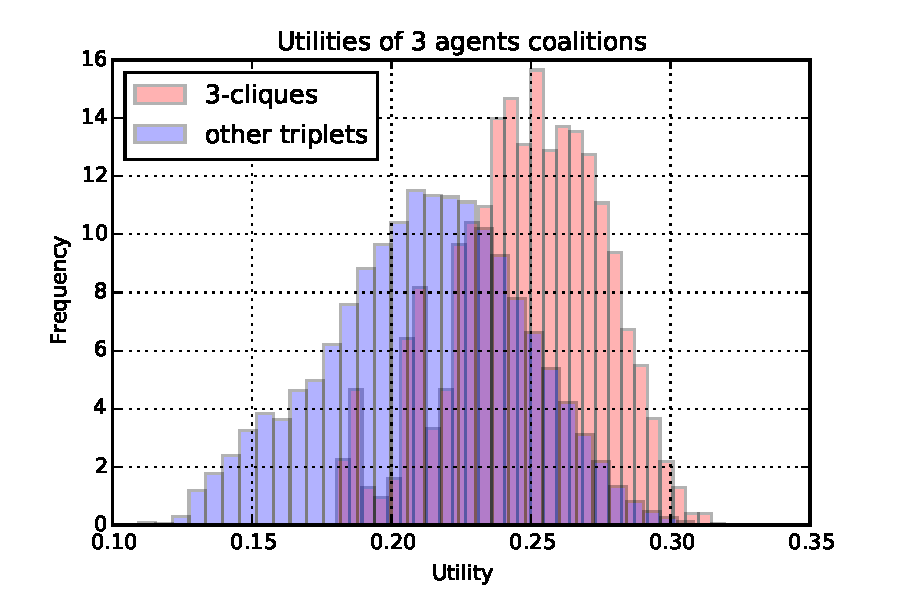
\includegraphics[scale=.6]{cliques_histo.pdf}
\caption{Histograms of utility values for coalitions of size 3. Red bars stands for cliques in the decorrelation graph, and blue bars represents all the other possible triplets. As visible, cliques tend to exhibit higher utilities than randomly selected coalitions.}
\label{fig:histo_cliques}
\end{figure}

Figure \ref{fig:histo_cliques} shows the distributions of the utility values for cliques of size 3 (triangles) in $ G_{2}^{\epsilon^{\star}} $ and for all the other possible triplets of agents. It is clearly visible that cliques tend to exhibit higher utilities because of their de-correlation property. Choosing cliques in $ G_{2}^{\epsilon^{\star}} $ as coalitions seems therefore appealing. Nevertheless, the quality of the results seems to decrease as the sizes of the cliques increase. Indeed, the larger the desired cliques, the more dense $ G_{2}^{\epsilon^{\star}} $ becomes (see equation \ref{epsilon_star}). There is a point where cliques results more from noisy edges than true de-correlation relationships, which decreases the quality of the results.

Directly mapping cliques to coalitions by this de-correlation oriented approach is thus not sufficient. It is indeed possible that adding agents to these cliques has the combined effect of increasing the expected production while decreasing its stability. The question revolves around measuring the benefits of this production surplus compared to the disadvantage of a higher unstability. This can be quantified by the marginal benefit of equation \ref{eq:marginal_benefit}.


\subsection{Coalition formation algorithm}

The algorithm takes inputs from :
\begin{itemize}
	\item \textbf{The agents :} historical series of available productions $P_{i}$, 
	\item \textbf{The grid operator :} market entrance policy $ (P^{MIN},\phi) $,
	\item \textbf{The "user" :} Number of desired coalitions $ N_{COAL} $ and size of starting cliques k.
\end{itemize} 
The first steps consists in computing the de-correlation graph $ G_{2} $ as well as the optimal threshold $ \epsilon^{\star} $. Cliques of size k in $ G_{2}^{\epsilon^{\star}} $ are considered as coalition seeds. The next step is a local greedy improvement over the correlation structure represented by  $ G_{2}^{\epsilon^{\star}} $. Cliques add alternatively the node $ i^{\star} $ in their neighborhood that yields the best marginal benefit $ MAX_{ i \in N(clique) } \delta_{clique}(i) $ where $ N(clique) $ is the neighborhood of a given clique. This addition occurs only if $ i^{\star} $ is not already involved in another coalition, and if $ \delta_{clique}(i^{\star}) \geq 0 $, meaning that utilities are increasing. The algorithm stops when all nodes are distributed in a coalition or when the global utility stops increasing. See the details in algorithm \ref{alg:algo1}.

\begin{algorithm}
 \KwData{$P_{i}$ series,\\ Grid policy $ (P^{MIN},\phi) $,\\ Desired number of coalitions $ N_{COAL} $,\\ size of starting cliques k}
 \KwResult{ $ CS = \{ S_{1},...,S_{N_{COAL}}\} $ }
 Compute $ G_{2}^{\epsilon^{\star}} $ \;
 Find the $ N_{COAL} $ cliques in $ G_{2}^{\epsilon^{\star}} $\;
 \While{$ \mathcal{U}(CS) $ is improving}{
 	\For{each clique}{
 		Find $ i^{\star} $ \;
 		\If{ $ \delta_{clique}(i^{\star}) >= 0 $ }{
 			$ clique \leftarrow clique \cup \{i^{\star} \} $ \;
 			}
   		}
  	}
 \caption{Percolation algorithm}
 \label{alg:algo1}
\end{algorithm}

\begin{algorithm}
 \KwData{Agent set $\mathcal{A}$,\\ Desired number of coalitions $ N_{COAL} $, \\ Maximum number of iterations $ maxiter $}
 \KwResult{ $ CS = \{ S_{1},...,S_{N_{COAL}}\} $ }
 $ curriter \leftarrow 0 $ \;
 $ CS^{\star} \leftarrow \emptyset $\;
 \While{$ curriter < maxiter $}{
 	$ CS \leftarrow SelectRandomCS() $\;
 	\If{ $ \mathcal{U}(CS) > \mathcal{U}(CS^{\star}) $ }{
 		$ CS^{\star } \leftarrow CS $\;
 		}
 	$ curriter \leftarrow  curriter + 1 $\;
  	}
  return $ CS^{\star} $
 \caption{Random algorithm}
 \label{alg:algo2}
\end{algorithm}

\begin{algorithm}
 \KwData{$P_{i}$ series,\\ Desired number of coalitions $ N_{COAL} $,\\ search step size $ \beta << 1 $}
 \KwResult{ $ CS = \{ S_{1},...,S_{N_{COAL}}\} $ }
 $ \epsilon \leftarrow 1 $ \;
 $ CS \leftarrow \emptyset $\;
 \While{$ |CS| < N_{COAL} $}{
 	Compute $ G_{1}^{\epsilon} $ \;
 	$ CS \leftarrow computeClusters( G_{1}^{\epsilon} ) $\;
 	\If{ $ |CS| = N_{COAL} $ }{
 		return CS\;
 		}
 	\Else{ 
 	$ \epsilon \leftarrow \epsilon - \beta $\;
 	}
  	}
 \caption{Correlated algorithm}
\label{alg:algo3}
\end{algorithm}

\section{Results}

The algorithm presented in the previous section is supposed to generate a given number of coalitions that have good utilities. Nevertheless, as it comprises mainly of a greedy optimization based on local improvements, the probability that the algorithm finds the optimal coalitions set is very low. Actually, it is not obvious that a strict optimum exists at all. Besides, there is, to our knowledge, no state of the art algorithm that aggregate uncorrelated agents in an optimum way (see section \ref{sec:related} for related problems in finance).


In order to have an idea about the algorithm's quality, we compare its results with :
\begin{itemize}
\item \textbf{Random :} This algorithm is basically a random search over the coalition structures space. It analyses a given number of structures and returns the best that it has encountered so far. See algorithm \ref{alg:algo2}.
\item \textbf{Correlated :} This is the complete opposite of our algorithm. It uses the correlation graph $ G_{1} $ and performs a community detection. The resulting coalitions have thus very high internal correlations. We thus expect this algorithm to perform very bad compared to the others. See algorithm \ref{alg:algo3}.
\end{itemize} 


Before running the algorithms, we need to calibrate the utility function by choosing the $ \alpha $ parameter. Recall that the purpose of this parameter is to take into account some constraints on the coalition's sizes if needed. In this paper, neither the communication network nor the electrical grid are explicitely considered. Thus, we do not have any technical constraints on coalition sizes even if we designed the utitility such that these could be taken into account. We select the desired size as being $ \lfloor N/N_{COAL} \rfloor $ (where $ \lfloor.\rfloor $ means floor). Figure \ref{fig:real_utility2} shows how the mean utility of a coalition evolves with its size when the optimum size is set to 40 agents. Using equation \ref{eq:alpha_star} to select $ \alpha $ based on the mean quantities seems to give acceptable results for the utility function.

Figure \ref{fig:search} displays the evolution of the global utility and the number of involved agents during the course of the greedy algorithm \ref{alg:algo1}. The transition from unvalid to valid coalitions is clearly visible on the blue diamond curve and occurs between iteration 10 and 15. After this transition, coalition's utilities improve slowly up to a maximum point. 

\begin{figure}
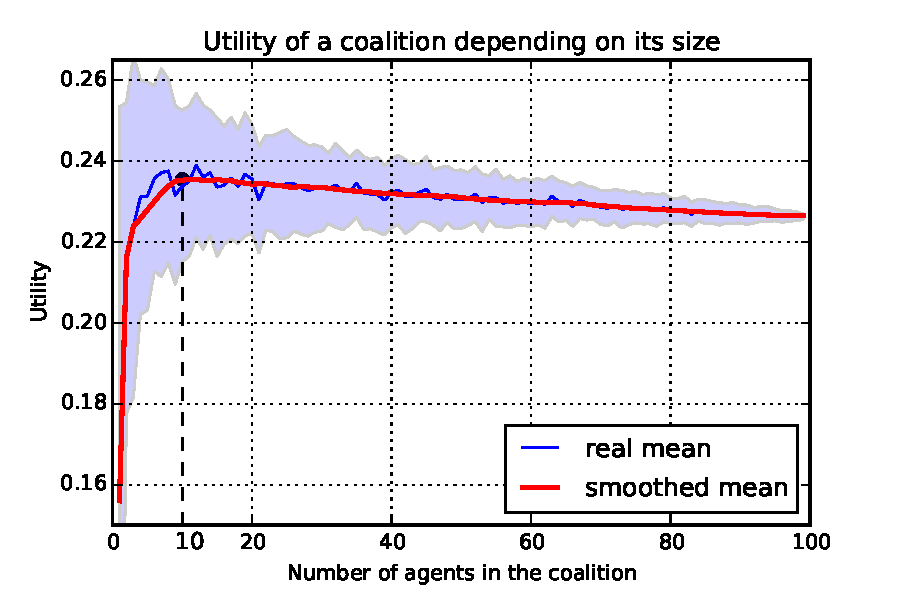
\includegraphics[scale=.6]{real_utility.pdf}
\caption{Utility of random coalitions depending on their size. Lines shows mean utility values and colored areas stands for standard deviations. The slim blue noisy curve shows the real mean utility, and the thick red curve is its smoothed version by applying a Savitzky-Golay filter. On this plot the $ \alpha $ parameter of the utility function was selected according to equation \ref{eq:alpha_star} in order to favor 10 agents coalitions.}
\label{fig:real_utility}
\end{figure}

\begin{figure}
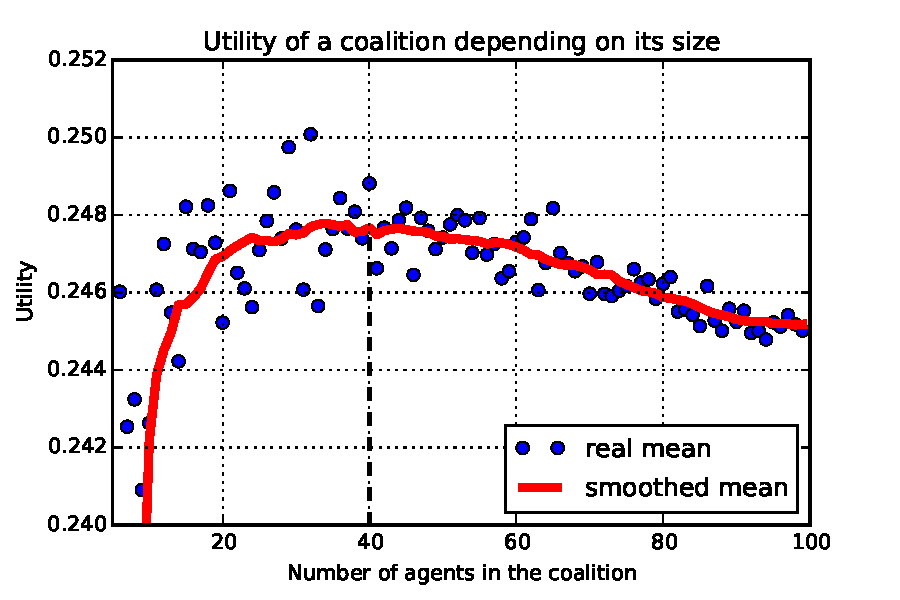
\includegraphics[scale=.6]{real_utility_2.pdf}
\caption{Utility of random coalitions depending on their size. Blue dots shows real mean utility values and the thick red curve its smoothed version by applying a Savitzky-Golay filter. On this plot the $ \alpha $ parameter of the utility function was selected according to equation \ref{eq:alpha_star} in order to favor 40 agents coalitions.}
\label{fig:real_utility2}
\end{figure}

\begin{figure}
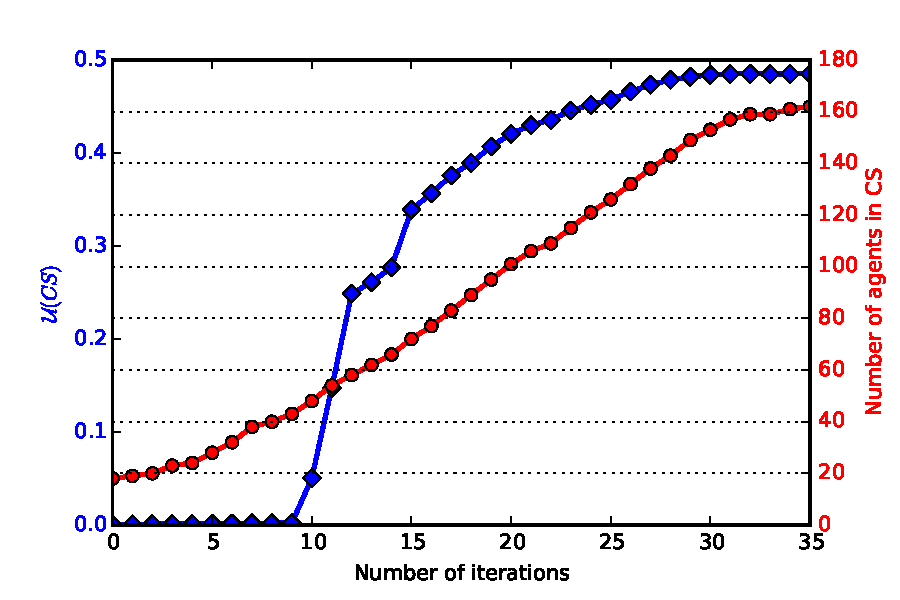
\includegraphics[scale=.6]{search.pdf}
\caption{Evolution of the global utility $ \mathcal{U}(CS) $ (blue diamond curve, left axis) and the number of agents involved in the coalitions (red circle curve, right axis) during the greedy optimization of algorithm \ref{alg:algo1} }
\label{fig:search}
\end{figure}


Figure \ref{fig:coalitions} shows the coalitions formed with the considered algorithms. A coalition is represented by a marker in the contract value / volatility space, and the color and shape of a marker indicates by which algorithm the coalition has been formed. Besides, as the size of a marker is proportional to the number of agents in the coalition, we can see that the utility function results in approximatively balanced coalitions. The coalitions of correlated agents (green squares) are clearly of poor quality according to our criteria since they can only afford small production contracts, and with a very high volatility (compared to the other coalitions on the plot). 

On figure \ref{fig:coalitions}, the de-correlated coalitions (blue dots) and the random ones (red triangles) are closer to the bottom right corner indicating a much better quality. We can see that, despite its simplicity, the random algorithm is able to achieve correct results thanks to the diversification inherent to such algorithm. Nevertheless, based on the utility, coalitions resulting from this random search are less good than the de-correlated ones. This can be understood on figure \ref{fig:coalitions} as the de-correlated coalitions are globally more located toward the bottom right corner, meaning that there are less disparities between coalitions than with the random case.


\begin{figure}
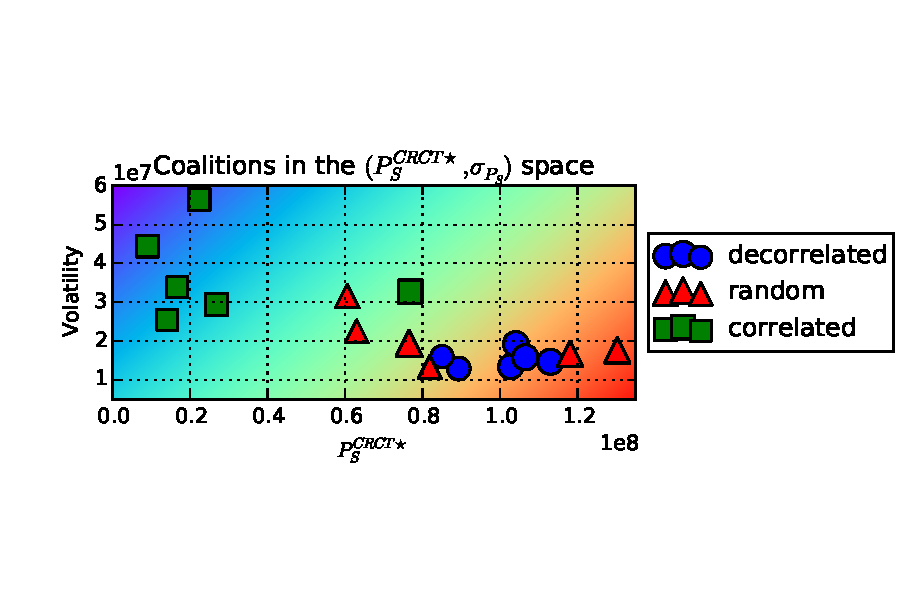
\includegraphics[scale=.6]{./figures/coalitions/coalitions.pdf}
\caption{Coalitions formed in the (contract value, volatility) space. The color map indicates qualities of portions of the plane. The closer to red the better (high contract values with small volatility). On the opposite, blue areas shows poor quality (small contract values with high volatility). Blue dots stand for the un-correlated coalitions, red triangles for random search, and green squares for correlated coalitions.}
\label{fig:coalitions}
\end{figure}

A key point for the coalitions, besides stability and productivity, is their resilience. The resilience of a system can be roughly described as its ability to perform its tasks when subject to failures of its components. Therefore, the notion of resilience we will use in the following can be seen as the ability of the coalition structures to inject stable power in the grid when node failures occur. According to our model, the grid operator specified two thresholds ($P^{MIN}$ and $ \phi $) such that the power injected by every coalition is constrained : $ P_{S}^{CRCT} \in [P^{MIN}, P_{S}^{CRCT \star}] $. As long as a coalition can propose a contract value higher than $ P^{MIN} $, it is valid and allowed to enter the energy market. We define the resilience of a coalition S as the probability that S produces more than the $ P^{MIN} $ threshold :

\begin{equation}
\mathcal{R}_{S} = 1 - Pr[P_{S} < P^{MIN}]
\end{equation}

And we extend this measure to the coalition stuctures :

\begin{equation}
\mathcal{R}_{CS} = \prod_{S \in CS} \left( 1 - Pr[ P_{S} < P^{MIN} ] \right)
\label{eq:resilience}
\end{equation}

We consider that prosumers fail randomly, and we denote by $ \psi \in [0,1] $ the fraction of agents that failed. Figure \ref{fig:resilience} exhibits how the resilience of the coalition structures evolve according to $ \psi $. On the top subplot, $ P^{MIN} $ was volontarily selected relatively low such that the resiliences of the three structures fit on the same figure. When the $ P^{MIN} $ requirement increases, the differences between the algorithms also increase as visible on the bottom subplot of figure \ref{fig:resilience}. The de-correlated coalitions seem to achieve a more resilient production on the market in the sense that they are able to sustain a higher fraction of node failures.

\begin{figure}
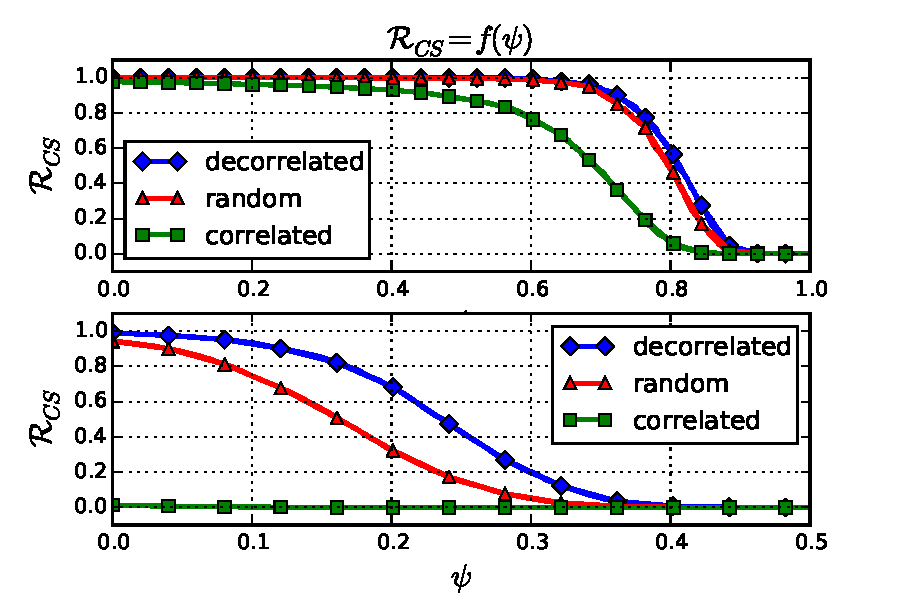
\includegraphics[scale=.6]{./figures/resilience_both.pdf}
\caption{Resilience of the coalition structures when nodes fail randomly (see equation \ref{eq:resilience}) for $ P^{MIN} = 10MW $ (top subplot) and $ P^{MIN} = 80MW $ (bottom subplot) }
\label{fig:resilience}
\end{figure}



%Let $ P^{MARKET} = \sum_{S \in CS} P_{S}^{CRCT} $ be the production on the market, where CS is the coalition structure formed $ CS = \{S_{1},...S_{N_{COAL}} \} $, and $ N_{COAL} $ is the number of coalitions in the structure. First of all, $ P^{MARKET} $ depends explicitely on $ N_{COAL} $ such that, forming more coalitions induces an increase of the production. However, for a finite pool of agents, we expect an optimal number of coalitions $ N_{COAL}^{\star} $ that maximizes the market production. The reason for this expectation is that, for a given number of agents, more coalitions causes necessarily less agents in the coalitions, and therefore less diversity. We expect thus a point where coalitions formed start to fail the market entrance, and deteriorate the market production.

%%%%%%%%%%%%%%%%%%%%%%%%%%%%%%%%%%%%%%%%%%%%%%%%%%%%%%%%%%%%%%%%%%%%%%%%%%%%%%%%
%
% Section VI: Conclusion
%
%%%%%%%%%%%%%%%%%%%%%%%%%%%%%%%%%%%%%%%%%%%%%%%%%%%%%%%%%%%%%%%%%%%%%%%%%%%%%%%%
\section{Conclusion}
\label{sec:conclusion}

In this paper we studied how aggregations of prosumers could be authorized to sell their surplus of production to the grid operator. By relying on the past values of the agents, we constrained the market entry to both sufficiently productive and stable coalitions. The power that a coalition is able to propose on the market is therefore related to both quantities. As the correlations between the prosumers that form these coalitions impact directly their volatilities, we seek uncorrelated aggregations of agents. We used a greedy algorithm that starts with cliques of the "de-correlation" graph of the agents and makes local improvements. We compare the results with a random search and an opposite strategy that clusters correlated agents together. We showed that the coalitions resulting from our algorithm are able to provide more stable power to the grid because they tend to have globally better production over volatility ratios while the others are generally more disparate. 

Because in real situations, agents are prone to failure, the resilience of the coalitions is an important criterium. We therefore studied how the coalitions are able to remain on the market when their agents fail randomly one by one. We showed that, in this situation, the coalitions resulting from our algorithm better withstand losses of agents.

%%%%%%%%%%%%%%%%%%%%%%%%%%%%%%%%%%%%%%%%%%%%%%%%%%%%%%%%%%%%%%%%%%%%%%%%%%%%%%%%
%
% Bibliography
%
%%%%%%%%%%%%%%%%%%%%%%%%%%%%%%%%%%%%%%%%%%%%%%%%%%%%%%%%%%%%%%%%%%%%%%%%%%%%%%%%
 
\bibliographystyle{IEEEtran}  
\bibliography{Article}


\end{document}


